\begin{frame}
	\frametitle{Biosphäre - Lebewesen}

	\begin{figure}
		\centering
		\includegraphics[trim={1cm 0cm 0cm 3cm}, clip, width=0.55\linewidth]{%
        bilder/climate_components/global_climate_components_biosphere.pdf}
		\caption{Die Vegetation ist eine interaktive Komponente des Klimasystems}
	\end{figure}

	\note{
		\begin{itemize}
			\item[] Umfasst sämtliches Leben auf der Erde
			\item[] Es zählen große Lebewesen, aber z.B. auch Mikroorganismen dazu
			\item[] Ersteckt sich von 5 km unter der Erdoberfläche bis etwa 60 km über der Erdoberfläche (eigentlich nichts ausgegraut in der Abbildung)
			\item[] Äußere Bereiche in großer Tiefe und Höhe ausschließlich von Mikroorganismen bewohnt.
			\item[] Läßt sich vielfach untergliedern in Ökozonen, Ökoregionen, Ökochore und Ökotope
			\item[] Vegetation ist sehr umfangreich und vielseitig
			\item[] bietet Lebensraum und Lebensgrundlage
			\item[] Die Erde besitzt die einzige uns bekannte Biosphäre
		\end{itemize}
	}
\end{frame}

\begin{frame}
	\frametitle{Biosphäre - Zonobiome}

	\begin{columns}
		\column{0.8\linewidth}
	    \begin{figure}
				\centering
				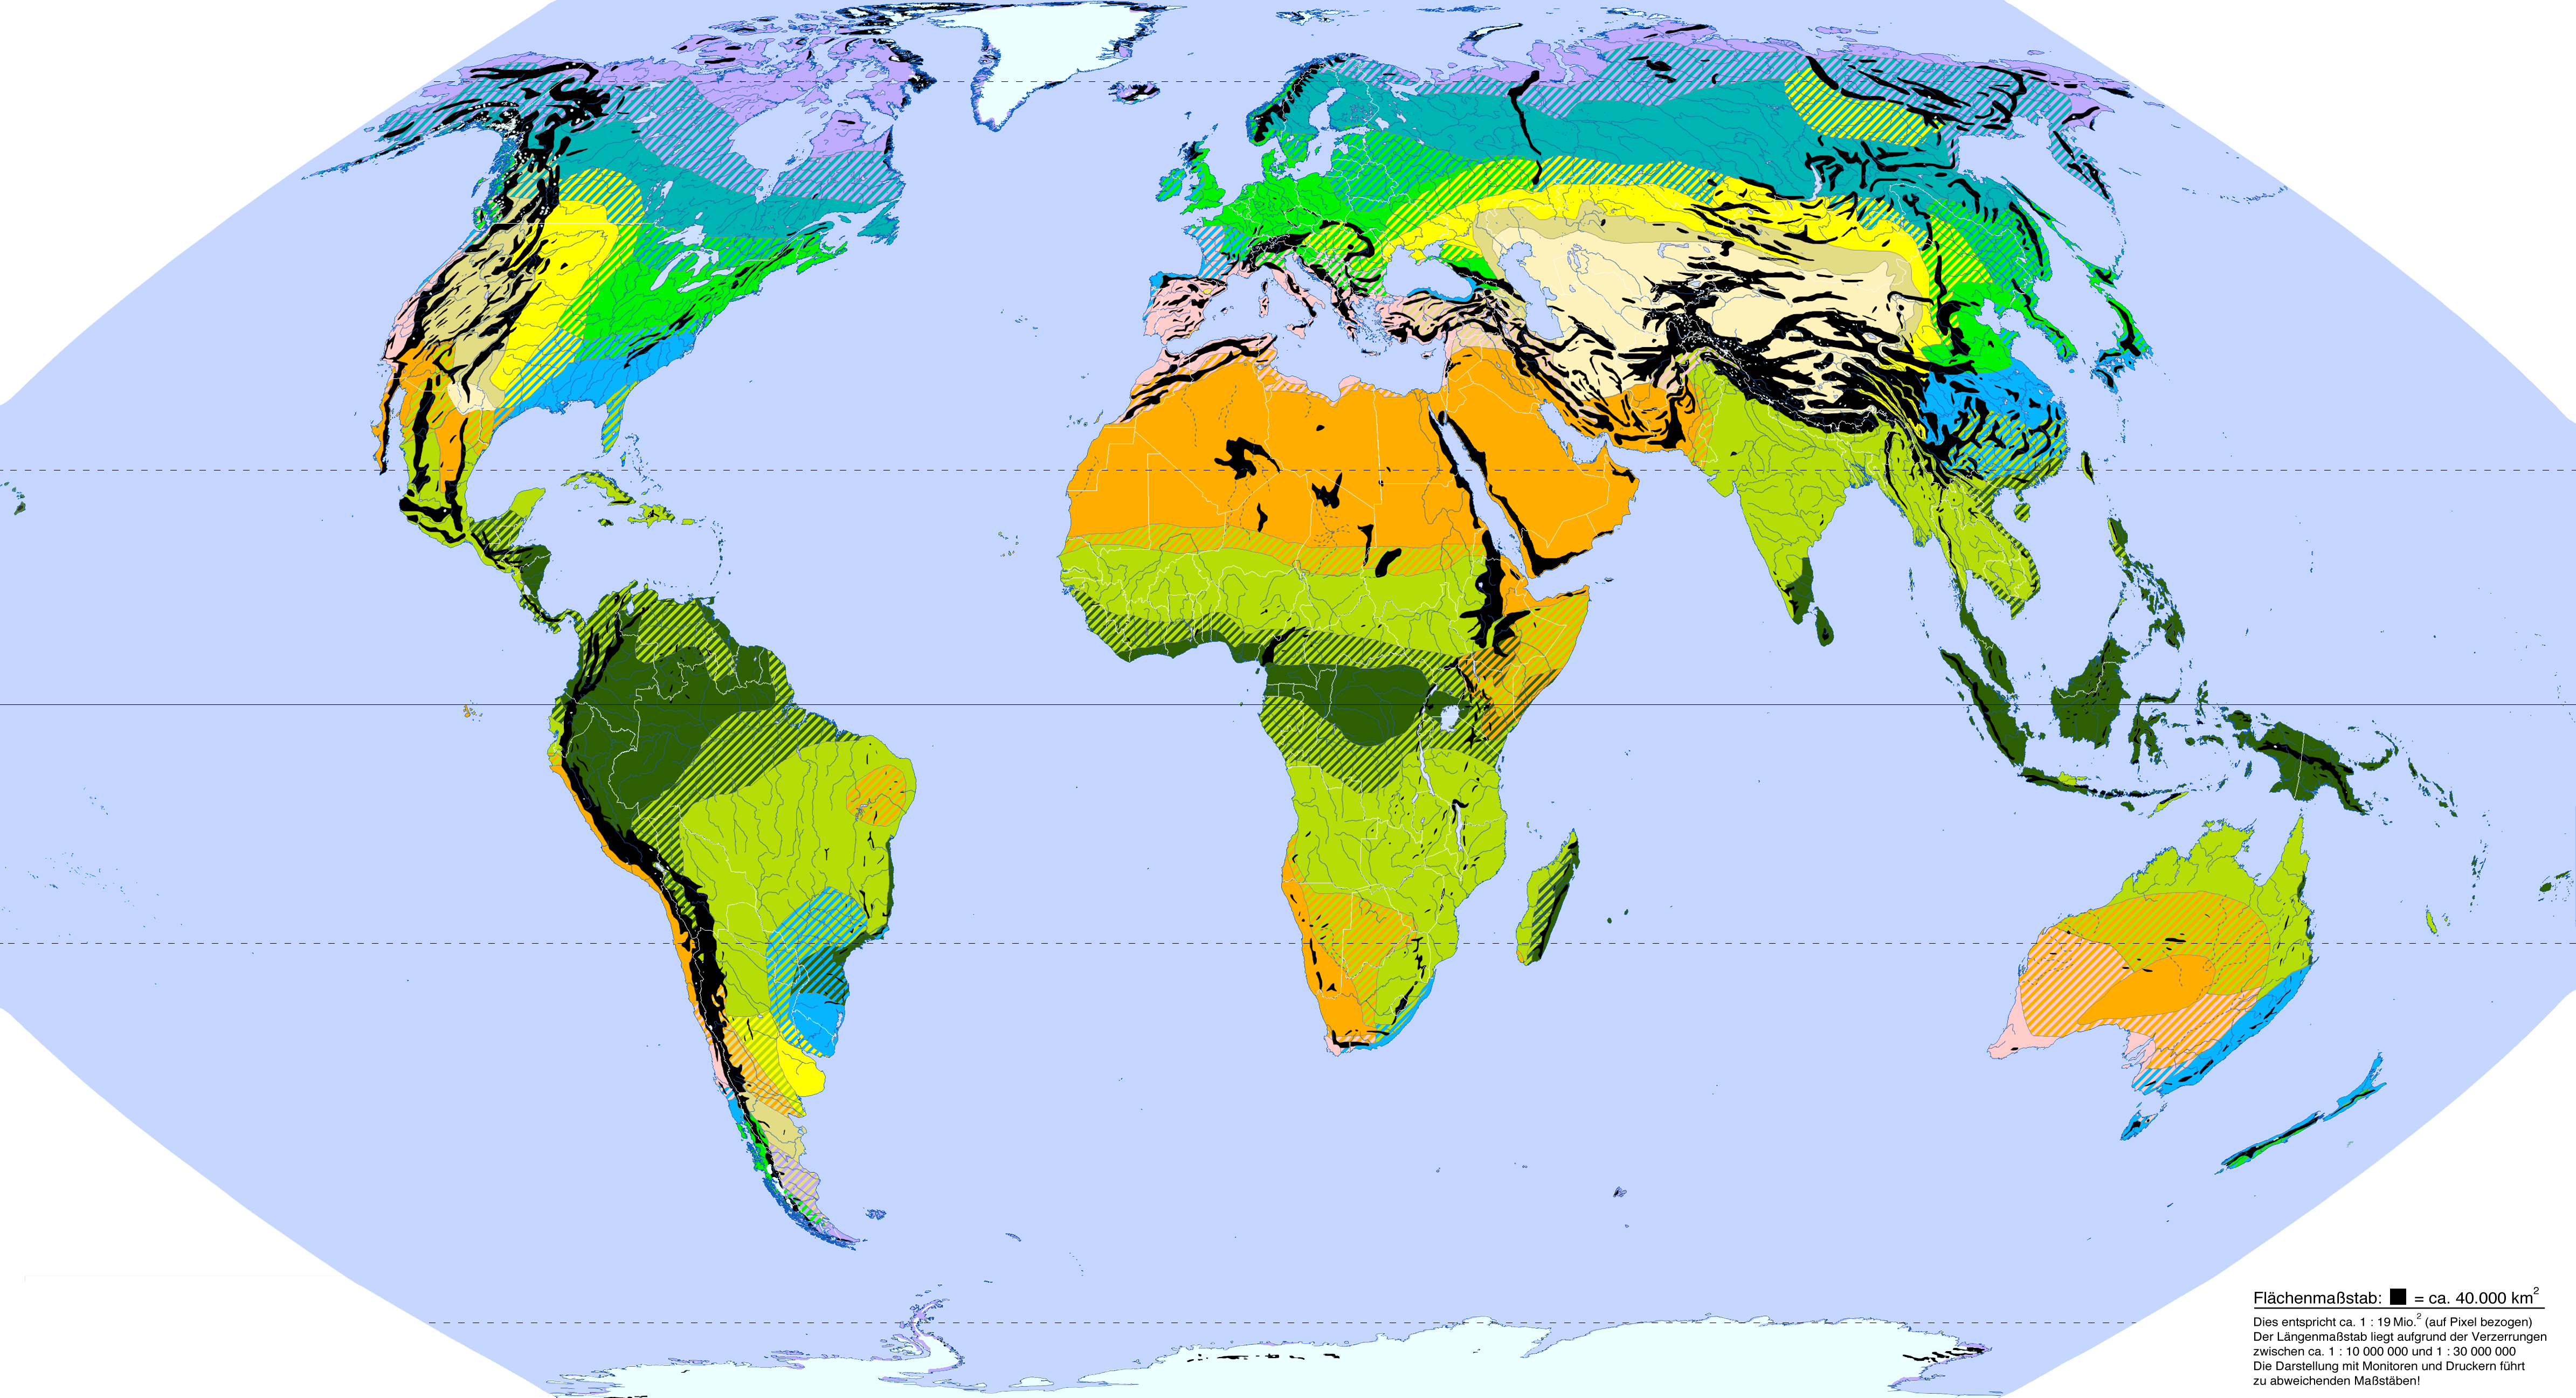
\includegraphics[width=\linewidth]{bilder/Zonobiome.png}
				\caption{Zonobiome und Zonoökotone (Übergangsräume) nach Walter und Breckle, Quelle: Wiki7}
			\end{figure}
		\column{0.2\linewidth}
		\begin{itemize}
			\item[\cbox{2d5f02}] ca. \SI{ 9}{\%}
      \item[\cbox{b7dd08}] ca. \SI{20}{\%}
			 \item[\cbox{ffae00}] ca. \SI{13}{\%}
      \item[\cbox{ffcccc}] ca. \SI{ 2}{\%}
      \item[\cbox{07b5ff}] ca. \SI{ 3}{\%}
      \item[\cbox{00f100}] ca. \SI{ 5}{\%}
			\item[\cbox{fdf2bb}] ca. \SI{ 4}{\%}
      \item[\cbox{e3dc84}] ca. \SI{ 3}{\%}
      \item[\cbox{ffff00}] ca. \SI{ 5}{\%}
      \item[\cbox{00b4b4}] ca. \SI{10}{\%}
      \item[\cbox{c0acfe}] ca. \SI{10}{\%}
      \item[\cbox{eafffe}] ca. \SI{ 5}{\%}
      \item[\cbox{000000}] ca. \SI{11}{\%}
		\end{itemize}
	\end{columns}

	\note{
	\begin{itemize}
		\item[]	Zonobiom: größere Übereinstimmungen in Klima, Vegetation, Tierwelt und Böden (hier 13)
		\item[] Die räumliche Lagebestimmung der Zonobiome richtet sich in erster Linie nach den Klimazonen.
		\item[] Ein Zonoökoton ist der Übergangsbereich zwischen zwei Zonobiomen.
		\begin{itemize}
			\item[\cbox{2d5f02}] I – tropische Regenwaldgebiete (ca. \SI{9}{\%})
      \item[\cbox{b7dd08}] II – tropisch-subtropische Regenzeitenwälder und Savannen (ca. \SI{20}{\%})
			 \item[\cbox{ffae00}] III – heiße Halbwüsten und Wüsten (ca. \SI{13}{\%})
      \item[\cbox{ffcccc}] IV – Mediterranes Zonobiom (Warmtemperate, dürre- und episodisch frostbelastete Gebiete mit Hartlaubwäldern) (ca. \SI{2}{\%})
      \item[\cbox{07b5ff}] V – Lorbeerwälder (Warmtemperate, regenreiche, episodisch frostbelastete Gebiete mit immergrünen Wäldern) (ca. \SI{3}{\%})
      \item[\cbox{00f100}] VI – Nemorales Zonobiom (Winterkalte Gebiete mit sommergrünen Wäldern) (ca. \SI{5}{\%})
			\item[] VII Wüsten und Steppen (ca. \SI{12}{\%})
			\item[\cbox{fdf2bb}] VII a) – Winterkalte Vollwüsten (ca. \SI{4}{\%})
      \item[\cbox{e3dc84}] VII b) – Winterkalte Halbwüsten (ca. \SI{3}{\%})
      \item[\cbox{ffff00}] VII c) – Winterkalte Steppen (ca. \SI{5}{\%})
      \item[\cbox{00b4b4}] VIII – Winterkalte Nadelwaldgebiete (ca. \SI{10}{\%})
      \item[\cbox{c0acfe}] IX – Tundren und polare Wüsten (ca. \SI{10}{\%})
      \item[\cbox{eafffe}] Eisschilde und Gletscher (ca. \SI{5}{\%})
      \item[\cbox{000000}] Gebirgszüge (Orobiome) (ca. \SI{11}{\%})
		\end{itemize}
		\item[] Nur die Biome auf der Erdoberfläche, in den Meeren ist noch wesentlich weniger verstanden. Auch hier hat jedes Biom Einfluss auf das Klima.
		\item[$\rightarrow$] Modellierung führt zu komplexen Klimamodellen
	\end{itemize}
	}
\end{frame}

\begin{frame}
	\frametitle{Biosphäre - Wechselwirkungen}
	\begin{columns}
		\column[t]{0.33\linewidth}
		\begin{figure}
			\centering
			\includegraphics[trim={0cm 0cm 0cm 0.1cm}, clip,width=\linewidth]{bilder/kuehe}
		\end{figure}
			\begin{itemize}
				\item Zahl der Tiere wirkt sich z.B. auf Methanausstoß aus
				\item Zahl der Tiere hängt vom Nahrungsangebot und menschlichem Einfluss ab
				\item Beweidung kann zu Albedoänderung führen
			\end{itemize}
		\column[t]{0.33\linewidth}
		\begin{figure}
			\centering
			\includegraphics[width=\linewidth]{bilder/plankton}
		\end{figure}
			\begin{itemize}
				\item Ozeane können CO$_2$ aufnehmen
				\item Kohlensäuregehalt wirkt sich auf Leben im Wasser aus
				\item Auch Lebewesen selbst beeinflussen Bedingungen
			\end{itemize}
		\column[t]{0.33\linewidth}
		\begin{figure}
			\centering
			\includegraphics[trim={0cm 0cm 0cm 3.8cm}, clip, width=\linewidth]{bilder/baeume}
		\end{figure}
			\begin{itemize}
				\item Pflanzen sind Kohlenstoffsenken
				\item Bewuchs wirkt sich auf Albedo aus
				\item Wälder haben starken Einfluss aus lokales Klima
			\end{itemize}
	\end{columns}

	\note{
		\begin{itemize}
			\item[] steht in direktem Kontakt mit unterer Atmosphäre und Böden durch photosynthetische Prozesse und die Aufnahme sowie Abgabe von Wasser
			\item[] Vegetation hat dadurch massiven Einfluss auf Wetter und Klima - z.B. Tropischer Regenwald, Wolkenbildung
			\item[] zentral ist auch die Rolle beim Stoffkreislauf - u.a. Kohlenstoff, Phosphor, Nitrat, Stickstoff (nächstes Mal)
		\end{itemize}
	}
\end{frame}
